% $HeadURL: https://sbgn.svn.sourceforge.net/svnroot/sbgn/trunk/documents/specifications/EntityRelationship/Level1/sources/glyphs.tex $

\chapter{Entity Relationship Glyphs}

[Note on the color code: \textcolor{blue}{The glyphs that have been thorougly discussed, and are considered frozen, are represented in blue}. \textcolor{green}{The glyphs that have been thorougly discussed, but are still posing problems are represented in green}. \textcolor{red}{The glyphs that have been proposed but for which in-depth discussion is yet to come are represented in red}.]

This chapter provides a catalog of the graphical symbols available for representing entities in \ER diagrams.  There are different classes of glyphs corresponding to different classes of entities, predicates, controls and operators.

%In \chap{grammar} beginning on page~\pageref{chp:grammar}, we describe the rules for combining these glyphs into a legal SBGN \ER, and in \chap{layout} beginning on page~\pageref{chp:layout}, we describe requirements and guidelines for the way that diagrams are visually organized.

\section{Overview}
 
% =============================================================================
% overview
% =============================================================================

To set the stage for what follows in this chapter, we first give a brief overview of some of the concepts in the \ER notation with the help of an example shown in \fig{eg1}. This example will be re-used throughout the description of the graphical symbols (glyphs) used by \SBGNERLone (with a few additions when the concepts are missing in the example) 

\begin{figure}[H]
  \centering
  \vspace*{-0.75em}
  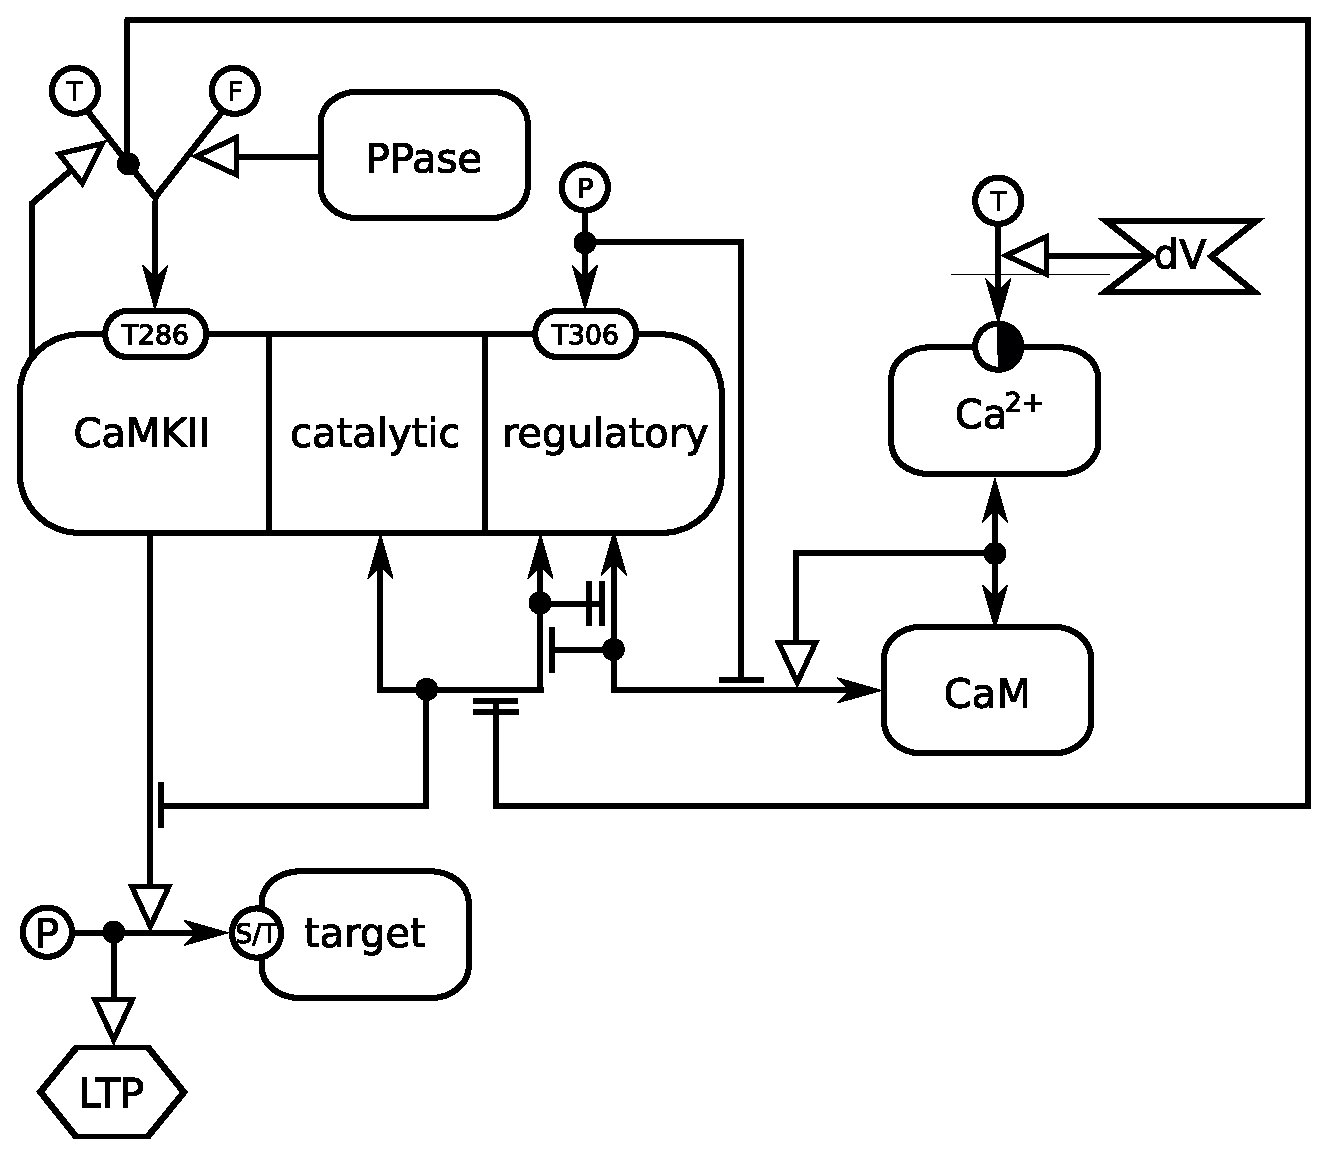
\includegraphics[scale=0.6]{examples/CaMKII-intro}
   \caption{This example of a \ER diagram depicts the effect of a depolarisation (dV) on the intracellular calcium, that binds to Calmodulin (CaM), that itself binds to the calcium/calmoduline kinase II (CaMKII). The binding of calmodulin inhibits the interaction between the catalytic and regulatory domains, thus relieving the inhibition on the kinase activity. The phosphorylation of the targets finally leads to the Long Term Potentiation (LTP) of the synapses. In addition, the diagram shows the effect of phosphorylation on threonine 286, that makes the enzyme constitutively active, and on threonine 306, that renders the kinase insensitive to calmodulin.}
  \label{fig:eg1}
\end{figure}
 
The essence of the \ER diagram is to depict the influences of entities upon the behaviour of others. The entities (in fact all interactors) are things that exist, either on their own or when statements become true. For instance, an entity can exist, different entities can interact, or a value can be assigned to an entity's property. The influences can therefore be understood as logical consequences of this existence. Contrary to the Process Diagram notation, where the different processes affect each other, the relationships are independent. On can imagine that each of the relationships represent a specific conclusion of a scientific experience or article. Their addition on a map represent the extend a the knowledge we have of the effects of the entities represented upon each other. The independence of relationships is the key to avoid the combinatorial explosion inherent to Process Diagrams.

\tab{component-summary} summarizes the different SBGN abstractions described in this chapter.
 
\newcolumntype{P}[1]{>{\raggedright\hspace{0pt}\arraybackslash}p{#1}}
 
 \begin{table}[h]
   \centering
   \small
   \begin{tabular}{@{}lP{2.4in}P{2.4in}@{}}
     \toprule
     \textbf{Component} & \textbf{Role} & \textbf{Examples}\\
     \midrule
     Interactor node
     & Something that exists
     & An entity, the result of an interaction \\[0.5em]
 
     Statement	
     & Something that can be true or false
     & An interaction between entities, the assignment of a value to a variable \\[0.5em]
 
     Influence
     & The effect of something true on the realisation of a statement or another influence.
     & A stimulation, an absolute inhibition \\
     \bottomrule
   \end{tabular}
   \caption{Summary of \ER components and their roles.}
   \label{tab:component-summary}
 \end{table}


 
\section{Controlled vocabularies used in \SBGNERLone}\label{sec:CVs}

%%%%%%%%%%%%%%%%%%%%%%%%%%%%%%%%%%%%%%%%%%%%%%%%%%%%%%%%%%%%%%%%%%%%%%%
%%%%                   Controlled vocabularies
%%%%%%%%%%%%%%%%%%%%%%%%%%%%%%%%%%%%%%%%%%%%%%%%%%%%%%%%%%%%%%%%%%%%%%

\section{Controlled vocabularies used in \SBGNERLone}\label{sec:CVs}

Some glyphs in SBGN \ERs can contain particular kinds of textual annotations conveying information relevant to the purpose of the glyph.  These annotations are carried by \glyph{units of information} (\sect{unitInformation}) or \glyph{state variable values} (\sect{stateVariable}).

The text that appears as the unit of information decorating an entity must be prefixed with a controlled vocabulary term indicating the type of information being expressed.  The prefixes are mandatory.  Without the use of controlled vocabulary prefixes, it would be necessary to have different glyphs to indicate different classes of information; this would lead to an explosion in the number of symbols needed.

In the rest of this section, we describe the controlled vocabularies (CVs) used in \SBGNERLone.  In each case, some CV terms are predefined by SBGN, but unless otherwise noted, \emph{they are not the only terms permitted}.  Authors may use other CV values not listed here, but in such cases, they should explain the terms' meanings in a figure legend or other text accompanying the map.

\subsection{Entity material types}
\label{sec:material-types-cv}

The material type of an \glyph{Entity} indicates its chemical structure.  A list of common material types is shown in \fig{material-types-cv}, but others are possible.  The values are to be taken from the \sbo (\sbourl), specifically from the branch having identifier \sboid{SBO:0000240} (\emph{material entity}).  The labels are defined by \SBGNERLone.

\begin{figure}[h]
  \centering
  \begin{tabular}{l>{\ttfamily}ll}
    \toprule
    \textbf{Name}              & \textbf{\rmfamily Label} & \textbf{SBO term} \\
    \midrule
    Non-macromolecular ion     & mt:ion  & SBO:0000327\\
    Non-macromolecular radical & mt:rad  & SBO:0000328\\
    Ribonucleic acid           & mt:rna  & SBO:0000250\\
    Deoxribonucleic acid       & mt:dna  & SBO:0000251\\
    Protein                    & mt:prot & SBO:0000297\\
    Polysaccharide             & mt:psac & SBO:0000249\\
    \bottomrule
  \end{tabular}
  \caption{A sample of values from the \emph{material types} controlled
    vocabulary (\sect{material-types-cv}).}
  \label{fig:material-types-cv}
\end{figure}

The material types are in contrast to the \emph{conceptual types} (see below).  The distinction is that material types are about physical composition, while conceptual types are about functions.  For example, a strand of RNA is a physical artifact, but its use as messenger RNA is a function.

\subsection{Entity conceptual types}
\label{sec:conceptual-types-cv}

An \glyph{entity}'s \emph{conceptual type} indicates its function within the context of a given \ERm.  A list of common conceptual types is shown in \fig{conceptual-types-cv}, but others are possible.  The values are to be taken from the \sbo (\sbourl), specifically from the branch having identifier \sboid{SBO:0000241} (\emph{functional entity}).  The labels are defined by \SBGNERLone.

\begin{figure}[h]
  \centering
  \begin{tabular}{l>{\ttfamily}ll}
    \toprule
    \textbf{Name}              & \textbf{\rmfamily Label} & \textbf{SBO term} \\
    \midrule
    Gene                      & ct:gene   & SBO:0000243\\
    Transcription start site  & ct:tss    & SBO:0000329\\
    Gene coding region        & ct:coding & SBO:0000335\\
    Gene regulatory region    & ct:grr    & SBO:0000369\\
    Messenger RNA             & ct:mRNA   & SBO:0000278\\
    Functional domain         & ct:domain & SBO:0000493\\
    Binding site              & ct:bind   & SBO:0000494\\
    Catalytic site            & ct:cat    & SBO:0000495\\
    Transmembrane domain      & ct:tm     & SBO:0000496\\
    \bottomrule
  \end{tabular}
  \caption{A sample of values from the \emph{conceptual types} vocabulary
    (\sect{conceptual-types-cv}).}
  \label{fig:conceptual-types-cv}
\end{figure}

\subsection{Macromolecule covalent modifications}
\label{sec:covalent-mod-cv}

A common reason for the introduction of state variables on an entity is to allow access to the configuration of possible covalent modification sites on that entity.  For instance, a macromolecule may have one or more sites where a phosphate group may be attached; this change in the site's configuration (\ie being either phosphorylated or not) may factor into whether, and how, the entity can participate in different processes.  Being able to describe such modifications in a consistent fashion is the motivation for the existence of SBGN's covalent modifications controlled vocabulary.  

\fig{covalent-mod-cv} lists a number of common types of covalent modifications.  The most common values are defined by the \sbo in the branch having identifier \sboid{SBO:0000210} (\emph{addition} under \emph{events}$\rightarrow$\emph{reaction}$\rightarrow$\emph{biochemical reaction}$\rightarrow$\emph{conversion}$\rightarrow$\emph{addition}).  The labels shown in \fig{covalent-mod-cv} are defined by \SBGNERLone; for all other kinds of modifications not listed here, the author of an \ERm must create a new label (and should also describe the meaning of the label in a legend or text accompanying the map).

\begin{figure}[h]
  \centering
  \begin{tabular}{l>{\ttfamily}ll}
    \toprule
    \textbf{Name}   & \textbf{\rmfamily Label} & \textbf{SBO term} \\
    \midrule
    Acetylation     & Ac    & SBO:0000215\\
    Glycosylation   & G     & SBO:0000217\\
    Hydroxylation   & OH    & SBO:0000233\\
    Methylation     & Me    & SBO:0000214\\
    Myristoylation  & My    & SBO:0000219\\
    Palmytoylation  & Pa    & SBO:0000218\\
    Phosphorylation & P     & SBO:0000216\\
    Prenylation     & Pr    & SBO:0000221\\
    Protonation     & H     & SBO:0000212\\
    Sulfation       & S     & SBO:0000220\\
    Ubiquitination  & Ub    & SBO:0000224\\
    \bottomrule
  \end{tabular}
  \caption{A sample of values from the \emph{covalent modifications} vocabulary
    (\sect{covalent-mod-cv}).}
  \label{fig:covalent-mod-cv}
\end{figure}

\subsection{Miscellaneous terms}
\label{sec:miscellaneous-cv}

\SBGNERLone requires several reserved characters. A special unit of information usable on interactions describe the number of identical interactors involved. Note that the value is a unitary number, and not (for example) a range.  There is no provision in \SBGNPDLone for specifying a range in this context because it leads to problems of entity identifiability. Other reserved characters are used in state variable assignments to represent truth or falsehood. Two reserved words are used in units of information carried by relationships: cis and trans. 

\begin{table}[h]
  \centering
  \begin{tabular}{l>{\ttfamily}l>{\ttfamily}l}
    \toprule
    \textbf{Name}   & \textbf{\rmfamily Label} & \textbf{\rmfamily SBO term} \\
    \midrule
    cardinality    & \#  & SBO:0000364\\
    true           & T     & SBO:0000416\\
    false          & F     & SBO:0000417\\
    cis            & cis   & SBO:0000414\\
    trans          & trans & SBO:0000415\\
    \bottomrule
  \end{tabular}
  \caption{Miscellaneous controlled terms. For the cardinality, \texttt{\#} stands for a number, for example, ``\texttt{5}''.}
  \label{tab:cardinality-cv}
\end{table}

%\normalcolor

 
 %%%%%%%%%%%%%%%%%%%%%%%%%%%%%%%%%%%%%%%%%%%%%%%%%%%%%%%%%%%%%%%%%%%%%%
 %%%%%%%%%%%%%%%%%%%%%%%%%%%%%%%%%%%%%%%%%%%%%%%%%%%%%%%%%%%%%%%%%%%%%%
 %%%%                   Entity nodes
 %%%%%%%%%%%%%%%%%%%%%%%%%%%%%%%%%%%%%%%%%%%%%%%%%%%%%%%%%%%%%%%%%%%%%%
 %%%%%%%%%%%%%%%%%%%%%%%%%%%%%%%%%%%%%%%%%%%%%%%%%%%%%%%%%%%%%%%%%%%%%%
 
 \section{Entity nodes}\label{sec:ENs}

% \SBGNERLone{} contains four glyphs representing classes of material entities: \glyph{unspecified entity}, \glyph{simple chemical}, \glyph{macromolecule} and \glyph{genetic entity}.  (Specific types of macromolecules, such as protein, RNA, DNA, polysaccharide, and specific simple chemicals are not defined by \SBGNERLone but may be part of future levels of SBGN.)  In addition to the material entities, \SBGNERLone{} represents five conceptual entities: \glyph{source/sink}, \glyph{perturbation}, \glyph{observable}, \glyph{tag} and \glyph{outcome}.  Material and conceptual entities can optionally carry auxiliary units such as \glyph{units of information} and \glyph{state variables}.
 

%% $HeadURL: https://sbgn.svn.sourceforge.net/svnroot/sbgn/trunk/documents/specifications/EntityRelationship/Level1/sources/unspecified.tex $

\color{red}

\subsection{Glyph: \glyph{Unspecified entity}}
\label{sec:unspecifiedEntity}

The simplest type of EN is the \glyph{unspecified entity}: one whose type is unknown or simply not relevant to the purposes of the model.  This arises, for example, when the existence of the entity has been inferred indirectly, or when the entity is merely a construct introduced for the needs of the model, without direct biological relevance.  These are examples of situations where the \emph{unspecified entity} glyph is appropriate.  (Conversely, for cases where the identity of the entities \emph{is} known, there exist other, more specific glyphs described elsewhere in the \SBGNERLone specification.)

\begin{glyphDescription}

\glyphSboTerm SBO:0000285 ! material entity of unknown nature 

\glyphContainer An \glyph{unspecified entity} is represented by an elliptic container, as shown in \fig{unspecified}.

\glyphLabel An \glyph{unspecified entity} is identified by a label placed in an unbordered box containing a string of characters.  The characters can be distributed on several lines to improve readability, although this is not mandatory.  The label box must be attached to the center of the container.  The label may spill outside of the container.

\end{glyphDescription}

\begin{figure}[H]
  \centering
  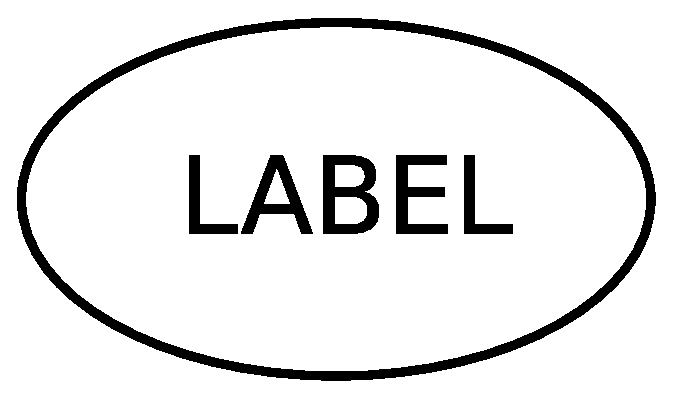
\includegraphics[scale = 0.3]{images/unspecified}
  \caption{The \ER glyph for \glyph{unspecified entity}.}
  \label{fig:unspecified}
\end{figure}

\normalcolor

% The following is for [X]Emacs users.   Please leave in place.
% Local Variables:
% TeX-master: "../sbgn_ER-level1"
% End:

%% $HeadURL: https://sbgn.svn.sourceforge.net/svnroot/sbgn/trunk/documents/specifications/EntityRelationship/Level1/sources/simpleChemical.tex $

\color{red}

\subsection{Glyph: \glyph{Simple chemical}}
\label{sec:simpleChemical}

A simple chemical in SBGN \ER is defined as the opposite of a macromolecule (\sect{macromolecule}): it is a chemical compound that is \emph{not} formed by the covalent linking of pseudo-identical residues.  Examples of simple chemicals are an atom, a monoatomic ion, a salt, a radical, a solid metal, a crystal, etc.

\begin{glyphDescription}

\glyphSboTerm SBO:0000247 ! simple chemical

\glyphContainer A \glyph{simple chemical} is represented by a circular container, as depicted in \fig{simpleChemical}.

\glyphLabel The identification of the \glyph{simple chemical} is carried by an unbordered box containing a string of characters.  The characters may be distributed on several lines to improve readability, although this is not mandatory.  The label box has to be attached to the center of the circular container.  The label is permitted to spill outside the container.

\glyphAux A \glyph{simple chemical} may be decorated with one or more \glyph{units of information} (\sect{unitInfo}).  A particular \glyph{unit of information} describes the material type.

\end{glyphDescription}

\begin{figure}[H]
  \centering
  
\includegraphics[scale = 0.3]{images/simpleChemical}
  \caption{The \ER glyph for \glyph{simple chemical}.}
  \label{fig:simpleChemical}
\end{figure}

\normalcolor

% The following is for [X]Emacs users.  Please leave in place.
% Local Variables:
% TeX-master: "../sbgn_ER-level1"
% End:

%\subsection{Glyph: \glyph{Macromolecule}}
\label{sec:macromolecule}

Many biological processes involve macromolecules: biochemical substances that are built up from the covalent linking of pseudo-identical units. Examples of macromolecules include proteins, nucleic acids (RNA, DNA), and polysaccharides (glycogen, cellulose, starch, etc.).  Attempting to define a separate glyph for all of these different molecules would lead to an explosion of symbols in SBGN, so instead, \SBGNERLone defines only one glyph for all macromolecules.  The same glyph is to be used for a protein, a nucleic acid, a complex sugar, and so on.  The exact nature of a particular macromolecule in a diagram is then clarified using its label and decorations, as will become clear below.  (Future levels of SBGN may subclass the \glyph{macromolecule} and introduce different glyphs to differentiate macromolecules.)

\begin{glyphDescription}

\glyphSboTerm SBO:0000245 ! macromolecule 

\glyphContainer A macromolecule is represented by a rectangular container with rounded corners, as illustrated in \fig{macromolecule}.

\glyphLabel A \glyph{macromolecule} is identified by a label placed in an unbordered box containing a string of characters.  The characters can be distributed on several lines to improve readability, although this is not mandatory.  The label box must be attached to the center of the container.  The label may spill outside of the container.

\glyphAux A \glyph{macromolecule} can carry state variables that can add information about its state (\sect{stateVariable}).  The state of a macromolecule is therefore defined as the vector of all its state variable values.  A state variable is represented by an ellipsoid container, with the long axis of the ellipsoid placed on the border of the \glyph{macromolecule}'s container as illustrated in \fig{macromolecule}.  The label of the state variable (which can precise the type of characteristic represented by the state variable, residue type, residue number etc.) is written within the state variable's container.

A \glyph{macromolecule} can also carry one or several \glyph{units of information} (\sect{unitInfo}).  The units of information can characterise a domain, such as a binding site.  Particular \glyph{units of information} are available for describing the material type (\sect{material-types-cv}) and the conceptual type (\sect{conceptual-types-cv}) of a macromolecule.  The center of the bounding box of a \glyph{unit of information} is located on the mid-line of the border of the macromolecule.

\end{glyphDescription}

\begin{figure}[H]
  \centering
  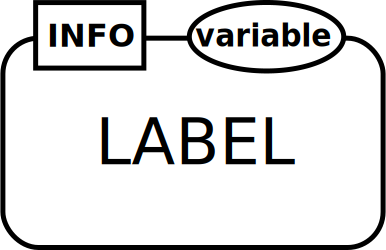
\includegraphics[scale = 0.3]{images/macromolecule}
  \caption{The \ER glyph for \glyph{macromolecule}.}
  \label{fig:macromolecule}
\end{figure}

\normalcolor
%% $HeadURL: https://sbgn.svn.sourceforge.net/svnroot/sbgn/trunk/documents/specifications/EntityRelationship/Level1/sources/genetic.tex $

\color{red}

\subsection{Glyph: \glyph{Genetic Entity}}
\label{sec:genetic}

The \emph{genetic entity} construct in SBGN is meant to represent a fragment of a macromolecule carrying genetic information.  A common use for this construct is to represent a gene or transcript.  The label of this EN and its \emph{units of information} are often important for making the purpose clear to the reader of a diagram.

\begin{glyphDescription}

\glyphSboTerm SBO:0000354 ! genetic entity

\glyphContainer A \glyph{genetic entity} is represented by a rectangular container whose bottom half has rounded corners, as shown in \fig{genetic}.

\glyphLabel The identity of a particular \glyph{genetic entity} is established by a label placed in an unordered box containing a string of characters.  The characters may be distributed on several lines to improve readability, although this is not mandatory.  The label box must be attached to the center of the container.  The label may spill outside of the container.

\glyphAux A \glyph{genetic entity} can carry state variables (\sect{stateVariable}) that add information about its precise state.  The state of a genetic entity is therefore defined as the vector of all its state variables.  A state variable is represented by an ellipsoid container, with the long axis of the ellipsoid placed on the border of the \glyph{genetic entity}'s container as illustrated in \fig{genetic}.  The label of the state variable (type of characteristic, nucleotide number) is written within the variable's container itself.

A \glyph{genetic information} can also carry one or several \glyph{units of information} (\sect{unitInfo}).  These can characterise a \glyph{genetic entity}'s domain, such as a binding site, or an exon.  Particular \glyph{units of information} carry the material type (\sect{material-types-cv}) and the conceptual type (\sect{conceptual-types-cv}) of the of the genetic entity.  The center of the bounding box of a \glyph{unit of information} is located on the mid-line of the border of the \glyph{genetic entity}.

\end{glyphDescription}


\begin{figure}[H]
  \centering
  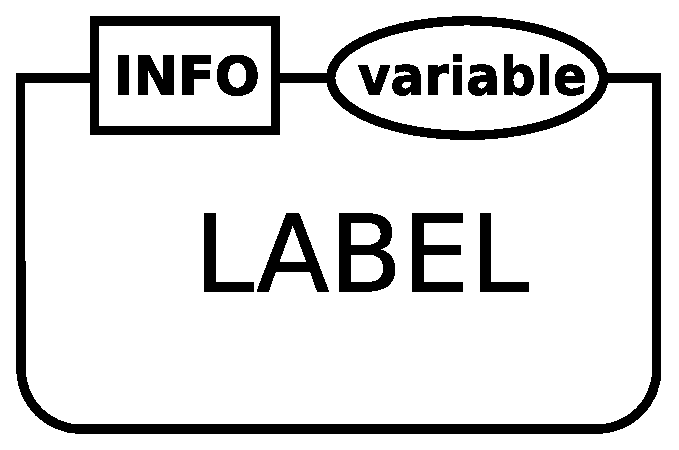
\includegraphics[scale = 0.3]{images/genetic}
  \caption{The \PD glyph for \glyph{genetic entity}.}
  \label{fig:genetic}
\end{figure}

\normalcolor

% The following is for [X]Emacs users.  Please leave in place.
% Local Variables:
% TeX-master: "../sbgn_ER-level1"
% End:


%% $HeadURL: https://sbgn.svn.sourceforge.net/svnroot/sbgn/trunk/documents/specifications/EntityRelationship/Level1/sources/sourceSink.tex $

\color{red}

\subsection{Glyph: \glyph{Source/sink}}
\label{sec:sourceSink}

It is useful to have the ability to represent the creation of an entity or
a state from an unspecified source, that is, from something that one does
not need or wish to make precise.  For instance, in a model where the
production of a protein is represented, it may not be desirable to
represent all of the amino acids, sugars and other metabolites used, or the
energy involved in the protein's creation.  Similarly, we may not wish to
bother representing the details of the destruction or decomposition of some
biochemical species into a large number of more primitive entities,
preferring instead to simply say that the species ``disappears into a
sink''.  Yet another example is that one may need to represent an input
(respectively, output) into (resp. from) a compartment without explicitly
representing a transport process from a source (resp. to a target).

For these and other situations, SBGN defines a symbol for explicitly
representing the involvement of an unspecified source or sink.  The symbol
used in SBGN is borrowed from the mathematical symbol for ``empty set'',
but it is important to note that it does not actually represent a true
absence of everything or a physical void---it represents the absence of the
corresponding structures in the model, that is, the fact that these sources
or sinks are conceptually outside the scope of the diagram.

A frequently asked question is, why bother having an explicit symbol at
all?  The reason is that one cannot simply use an arc that does not
terminate on a node, because the dangling end could be mistaken to be
pointing to another node in the diagram.  This is specially true if the
diagram is rescaled, causing the spacing of elements in the diagram to
change, and in the case of automatic layout.  The availability and use of an explicit symbol for sources and
sinks is therefore critical.

\begin{glyphDescription}

\glyphSboTerm SBO:0000291 ! empty set

\glyphContainer A \glyph{source/sink} is represented by a glyph for ``empty
set'', that is, a circle crossed by a bar linking the upper-right and
lower-left corners of an invisible square drawn around the circle.
\fig{sourceSink} illustrates this.  The symbol should only be linked to one
and only one edge in a diagram.

\glyphLabel An \glyph{source/sink} does not carry any labels.

\glyphAux An \glyph{source/sink} does not carry any auxiliary items.  

\end{glyphDescription}

\begin{figure}[H]
  \centering
  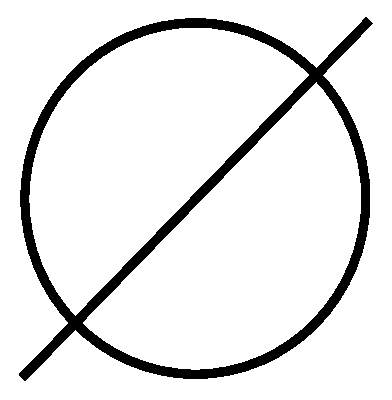
\includegraphics[scale = 0.3]{images/sourceSink}
  \caption{The \ER glyph for \glyph{source/sink}.}
  \label{fig:sourceSink}
\end{figure}

\normalcolor

% The following is for [X]Emacs users.    Please leave in place.
% Local Variables:
% TeX-master: "../sbgn_ER-level1"
% End:

%%%%%%%%%%%%%%%%%%%%%%%%%%%%%%%%%%%%%%%%%%%%%%%%%%%%%%%%%%%%%%%%%%%%%%%
%%                     Perturbing agent
%%%%%%%%%%%%%%%%%%%%%%%%%%%%%%%%%%%%%%%%%%%%%%%%%%%%%%%%%%%%%%%%%%%%%%
\color{red}

\subsection{Glyph: \glyph{Perturbing agent}}
\label{sec:perturbation}
 
Biochemical networks can be affected by external influences. Those
influences can be well-defined physical perturbations, such as a the effect of a light
pulse or of a change in temperature; they can also be more complex and not
well-defined phenomena, for instance a biological process, an experimental
setup, or a mutation.  For these situations, SBGN provides the
\glyph{perturbing agent} glyph. We do not use the word \emph{perturbation} to avoid the misunderstanding with the influence that the \glyph{perturbing agent} has on the map. 

\begin{glyphDescription}

\glyphSboTerm SBO:0000405 ! perturbing agent

\glyphContainer A \glyph{perturbing agent} is represented by a modified hexagon
having two opposite concave faces, as illustrated in \fig{perturbation}.

\glyphLabel A \glyph{perturbing agent} is identified by a label placed in an
unbordered box containing a string of characters.  The characters can be
distributed on several lines to improve readability, although this is not
mandatory.  The label box must be attached to the center of the
\glyph{perturbing agent} container.  The label may spill outside of the container.

\glyphAux A \glyph{perturbing agent} does not carry any auxiliary unit. [DOES-IT NOT? IS-IT AN ENTRY POINT? WHAT ABOUT THE EXISTENCE AND LOCATION VARIABLES?]

\end{glyphDescription}

\begin{figure}[H]
  \centering
  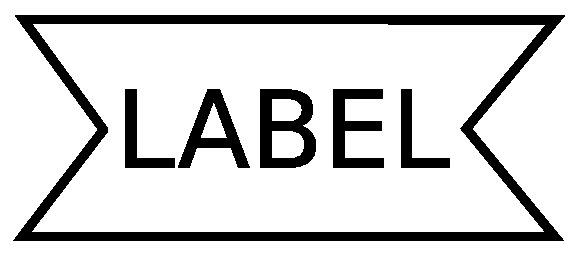
\includegraphics[scale = 0.3]{images/perturbation}
  \caption{The \ER glyph for \glyph{perturbing agent}.}
  \label{fig:perturbation}
\end{figure}

\begin{figure}[H]
  \centering
  \includegraphics[scale = 0.5]{examples/ex-perturbing}
  \caption{Example of a \glyph{perturbing agent} representing the depolarisation of a membrane, that stimulates (\sect{stimulation}) the existence (see \ref{sec:existence}) of an interactor.}
  \label{fig:ex-perturbing}
\end{figure}

\normalcolor

%
\color{red}

\subsection{Glyph: \glyph{Observable}}
\label{sec:observable}

A biochemical network can generate phenotypes or affect biological
processes.  Such processes can take place at different levels and are
independent of the biochemical network itself.  To represent these
processes in a diagram, SBGN defines the \glyph{observable} glyph.

\begin{glyphDescription}

\glyphSboTerm SBO:0000358 ! process that affects an observable

\glyphContainer An \glyph{observable} is represented by an elongated
hexagon, as illustrated in \fig{observable}.

\glyphLabel An \glyph{observable} is identified by a label placed in an
unbordered box containing a string of characters.  The characters can be
distributed on several lines to improve readability, although this is not
mandatory.  The label box must be attached to the center of the
\glyph{observable} container.  The label may spill outside of the container.

\textbf{DISCUSSION POINT HERE}

\glyphAux It is proposed that an \glyph{observable} glyph would stand as a short-hand for an entity representing the thing we measure, carrying a state variable existence (\sect{existence}). An \glyph{observable} would therefore be different than the other entities because modulatory arcs would directly connect to it, while none would origin from it.
\end{glyphDescription}
 
\begin{figure}[H]
  \centering
  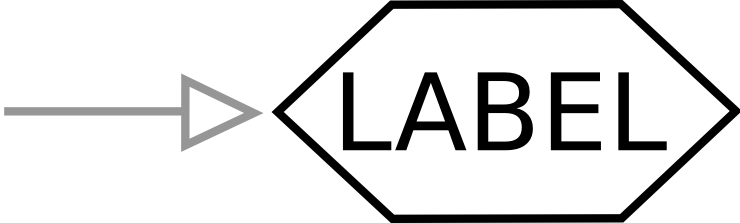
\includegraphics[scale = 0.3]{images/observable}
  \caption{The \ER glyph for \glyph{observable}.}
  \label{fig:observable}
\end{figure}

\normalcolor

% The following is for [X]Emacs users.   Please leave in place.
% Local Variables:
% TeX-master: "../sbgn_ER-level1"
% End:

%% $HeadURL: https://sbgn.svn.sourceforge.net/svnroot/sbgn/trunk/documents/specifications/EntityRelationship/Level1/sources/tag.tex $

\color{red}

\subsection{Glyph: \glyph{Tag}}
\label{sec:tag}

A \glyph{tag} is a named handle, or reference, to another EN (\sect{ENs}) or a container node (\sect{CNs}).  \glyph{Tags} can be used to identify elements in SBGN \glyph{submaps} (\sect{submap}).

\begin{glyphDescription}

\glyphSboTerm Not applicable.

\glyphContainer A \glyph{tag} is represented by a rectangle fused to an empty arrowhead, as illustrated in \fig{tag}.  The symbol should only be linked to one and only one edge (\ie it should reference only one EN or container).

\glyphLabel A \glyph{tag} is identified by a label placed in an unbordered box containing a string of characters.  The characters can be distributed on several lines to improve readability, although this is not mandatory.  The label box must be attached to the center of the container.  The label may spill outside of the container.

\glyphAux A \glyph{tag} does not carry any auxiliary items. 

\end{glyphDescription}

\begin{figure}[H]
  \centering
  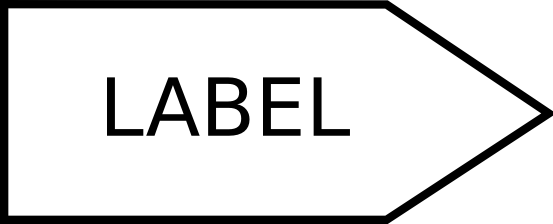
\includegraphics[scale = 0.3]{images/tag}
  \caption{The \ER glyph for \glyph{tag}.}
  \label{fig:tag}
\end{figure}

\normalcolor

% The following is for [X]Emacs users.   Please leave in place.
% Local Variables:
% TeX-master: "../sbgn_ER-level1"
% End:


%
%%%%%%%%%%%%%%%%%%%%%%%%%%%%%%%%%%%%%%%%%%%%%%%%%%%%%%%%%%%%%%%%%%%%%%
%%%%                   Outcome
%%%%%%%%%%%%%%%%%%%%%%%%%%%%%%%%%%%%%%%%%%%%%%%%%%%%%%%%%%%%%%%%%%%%%%
%\color{blue}
\subsubsection{Glyph: \glyph{Outcome}}\label{sec:outcome}

In \ERs, an \glyph{outcome} represents the actualisation of a \glyph{statement} (\sect{statements}). It is not entity on its own, but subset of all possible entity instances where \glyph{statement}  is true. For instance, if an \glyph{interaction} represents a non-covalent binding, the \glyph{outcome} represents all possible complexes that has two interactors bound to each other. If an \glyph{interaction} represents a genetic interaction, for instance derived from genetic screenings, the \glyph{outcome} represents the result of the presence of the two polymorphisms. If an \glyph{assignment} represents the phosphorylation of a protein, the \glyph{outcome} represents all possible complexes and free molecules where this protein is phosphorylated.

An \glyph{outcome} represent a particular instance of a realisation, and therefore, from one outcome must depart only one influence. An outcome being an \glyph{entity node}, it cannot receive influences. It exists. It cannot more or less exist. 

\begin{glyphDescription}

\glyphSboTerm SBO:0000409 ! interaction outcome

\glyphContainer  An \glyph{outcome} is represented by a black dot located on the arc of a \glyph{statement} (\sect{statements}). The diameter of the dot has to be larger than the thickness of the arc.

\glyphLabel An \glyph{outcome} has no identity on its own and does not carry any label. 

\glyphAux An \glyph{outcome} does not carry any auxiliary items.

\end{glyphDescription}

\begin{figure}[H]
  \centering
  
\includegraphics[scale = 0.5]{images/outcome}
  \caption{The \ER glyph for \glyph{outcome}.}
  \label{fig:outcome}
\end{figure}

\begin{figure}[H]
  \centering
  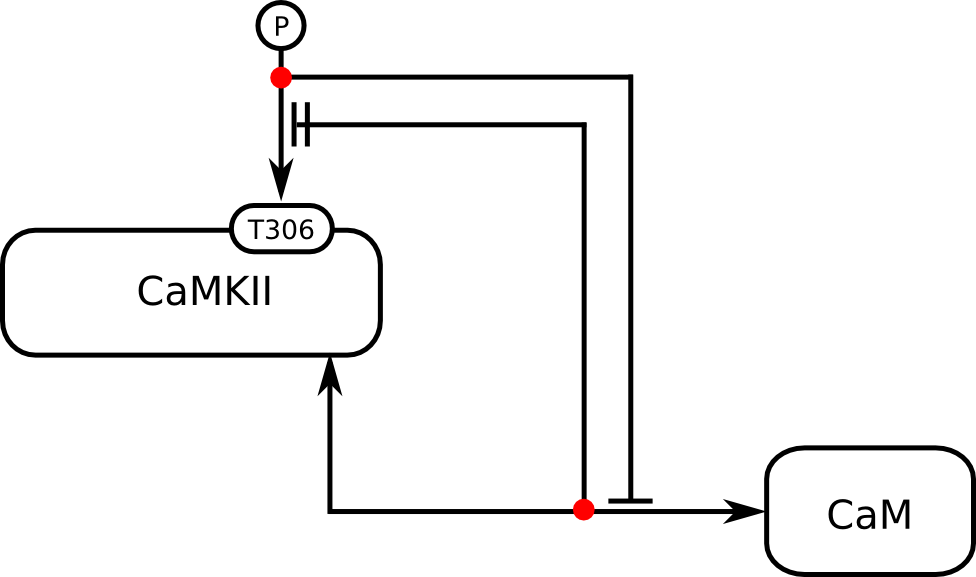
\includegraphics[scale = 0.5]{examples/ex-outcome}
  \caption{Examples of \glyph{outcomes}. The rightmost represents the fact that calmodulin effectively interacts (\sect{interaction}) with calcium/calmodulin kinase II. The leftmost represents the fact that the value phosphorylated is assigned (\sect{assignment}) to the variable representing threonin 306 of calcium/calmodulin kinase II.}
  \label{fig:ex-outcome}
\end{figure}

%\normalcolor
	


%%%%%%%%%%%%%%%%%%%%%%%%%%%%%%%%%%%%%%%%%%%%%%%%%%%%%%%%%%%%%%%%%%%%%%%
%%                     Unit of Information
%%%%%%%%%%%%%%%%%%%%%%%%%%%%%%%%%%%%%%%%%%%%%%%%%%%%%%%%%%%%%%%%%%%%%%
\color{blue}

\subsection{Glyph: \glyph{Unit of information}}
\label{sec:unitInformation}

When representing biological entities, it is often necessary to convey some abstract information about the entity's function or structure.  The SBGN \glyph{unit of information} is a decoration that can be used in this situation to add information to a glyph.  Some example uses of a \glyph{unit of information} include (but are not limited to) providing an identifier for an interaction, characterizing a logical part of an entity, information about the physical environment, or the specific type of biological entity it is decorating.

\begin{glyphDescription}

\glyphSboTerm Not applicable.

\glyphContainer A unit of information is represented by a rectangle.  The long side of the rectangle should be oriented parallel to the border of the \glyph{entity} being annotated by the \glyph{unit of information}. The center of the bounding box of a \glyph{state of information} should be located on the mid-line of the border of the \glyph{entity}.

\glyphLabel A \glyph{unit of information} is identified by a label placed in an unbordered box containing a string of characters.  The characters can be distributed on several lines to improve readability, although this is not mandatory.  The label box must be attached to the center of the container.  The label may spill outside of the container.

The label defines the information carried by the \glyph{unit of information}.  For certain predefined types of information having controlled vocabularies associated with them, SBGN defines specific prefixes that must be included in the label to indicate the type of information in question.  The controlled vocabularies predefined in \SBGNERLone are described in \sect{CVs} and summarized in the following list:

\begin{center}
  \begin{itemize}\setlength{\parskip}{0ex}
  \item[\texttt{mt}] entity material type
  \item[\texttt{ct}] entity conceptual type
  \end{itemize}
\end{center}

\glyphAux A \glyph{unit of information} does not carry any auxiliary items.

\end{glyphDescription}

\begin{figure}[H]
  \centering
  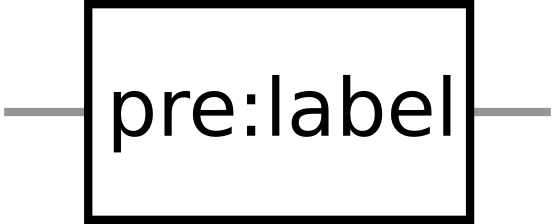
\includegraphics[scale = 0.3]{images/unitInformation}
  \caption{The \ER glyph for \glyph{unit of information}.}
  \label{fig:unitInformation}
\end{figure}

\begin{figure}[H]
  \centering
  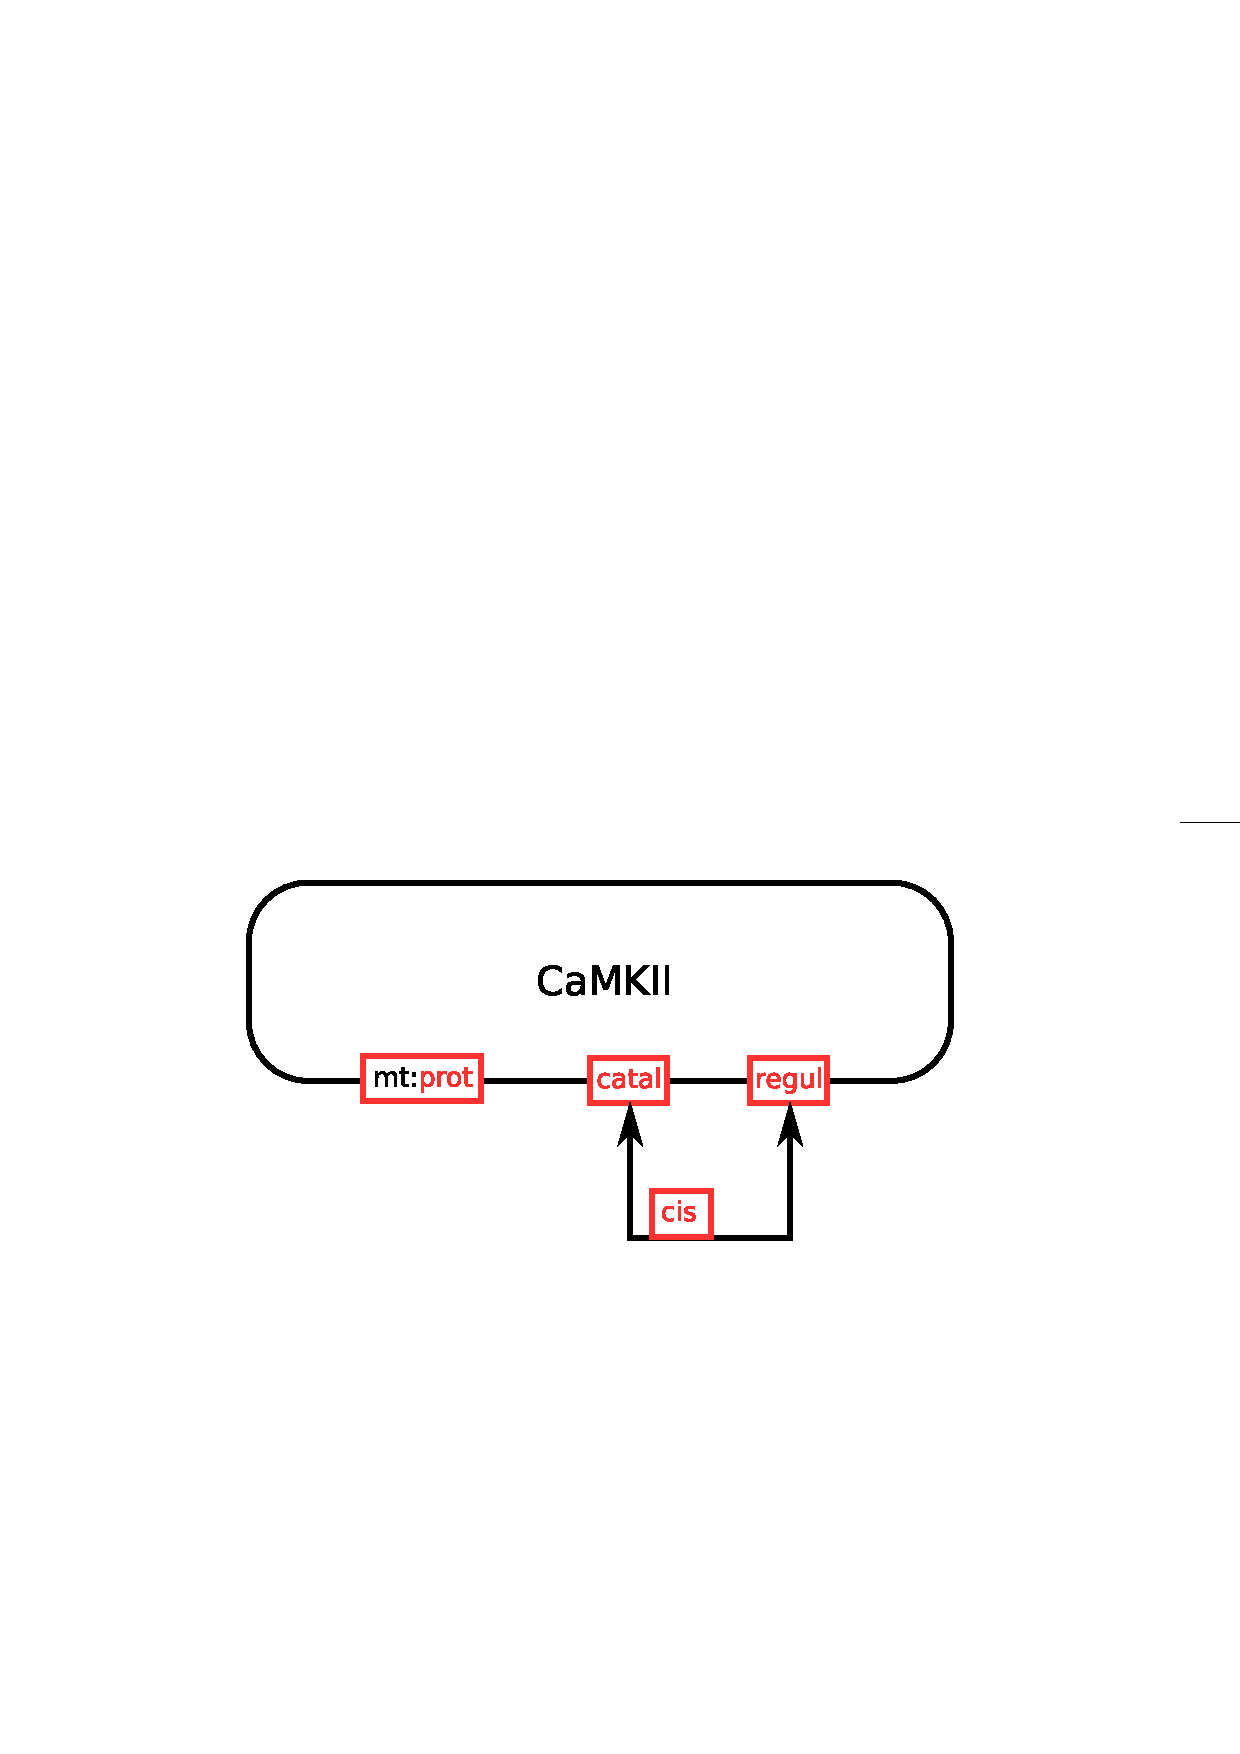
\includegraphics[scale = 0.5]{examples/ex-unitInformation}
  \caption{Using a \glyph{unit of information} to represent the fact that the entity ``CaMKII'' is a protein.}
  \label{fig:ex-unitInformation}
\end{figure}

\normalcolor

%%%%%%%%%%%%%%%%%%%%%%%%%%%%%%%%%%%%%%%%%%%%%%%%%%%%%%%%%%%%%%%%%%%%%%%
%%                     State variable
%%%%%%%%%%%%%%%%%%%%%%%%%%%%%%%%%%%%%%%%%%%%%%%%%%%%%%%%%%%%%%%%%%%%%%
%\color{blue}

\subsection{Glyph: \glyph{State variable}}
\label{sec:stateVariable}

Many biological entities such as molecules can exist in different \emph{states}, meaning different physical or informational configurations.  These states can arise for a variety of reasons.  For example, macromolecules can be subject to post-synthesis modifications, wherein residues of the macromolecules (amino acids, nucleosides, or glucid residues) are modified through covalent linkage to other chemicals.  Other examples of states are alternative conformations as in the closed/open/desensitized conformations of a transmembrane channel, and the active/inactive forms of an enzyme.

SBGN provides a means of associating one or more \glyph{state variables} with an entity; each such variable can be used to represent a dimension along which the state of the overall entity can vary.  When an entity can exist in different states, the state of the instance of the entity % (\ie the SBGN object) 
can be described by the current values of all its \glyph{state variables}, and the values of the \glyph{state variables} of all its possible components, recursively.

In \SBGNERLone, \glyph{state variables} are also used to describe the localisation in compartments (a transport is therefore described as a state variable assignment, see \sect{assignment}).

\begin{glyphDescription}

\glyphSboTerm Not applicable.

\glyphContainer A \glyph{state variable} is represented by a ''stadium'' container, that is two semicircles of same radius joined by parallel segments, as shown in \fig{state-var}.  The parallel segment axis should be tangent to the border of the glyph of the \glyph{entity} being modified by the \glyph{state variable}. The center of the bounding box of a \glyph{state variable} should be located on the mid-line of the border of the \glyph{entity}.

\glyphLabel A \glyph{state variable} is identified by a label placed in an unbordered box containing a string of characters.  The characters can be distributed on several lines to improve readability, although this is not mandatory.  The label box must be attached to the center of the container.  The label may spill outside of the container.

\glyphAux A \glyph{state variable} does not carry any auxiliary items.  

\end{glyphDescription}

\begin{figure}[H]
  \centering
  \includegraphics[scale = 0.3]{images/stateVariable}
  \caption{The \ER glyph for \glyph{state variable}. From left to right, horizontal \glyph{state variable}, vertical \glyph{state variable}, \glyph{location}, \glyph{existence}.}
  \label{fig:state-var}
\end{figure}

Two state variables are predefined. The variable \glyph{existence} is used to represent the creation or destruction of entities, as seen on \fig{ex-existence}\label{sec:existence}. \glyph{Existence} can take two values, true (T) or false (F). The variable is represented by a circle vertically divided in two. One hemicircle is black, and the other white. 

\begin{figure}[H]
  \centering
  \includegraphics[scale = 0.5]{examples/ex-existence}
  \caption{Using the \glyph{state variable} \glyph{existence} to represent the appearance of calcium following a depolarisation.}
  \label{fig:ex-existence}
\end{figure}

The variable \glyph{location} is used to represent the physical location of an entity, as seen on \fig{ex-location}\label{sec:location}. \glyph{Location} can take any value, but there can be only one \glyph{location} per instance of an entity. The variable is represented by a circle containing two perpendicular segments, an abstract version of the usual slanted pin.

\begin{figure}[H]
  \centering
  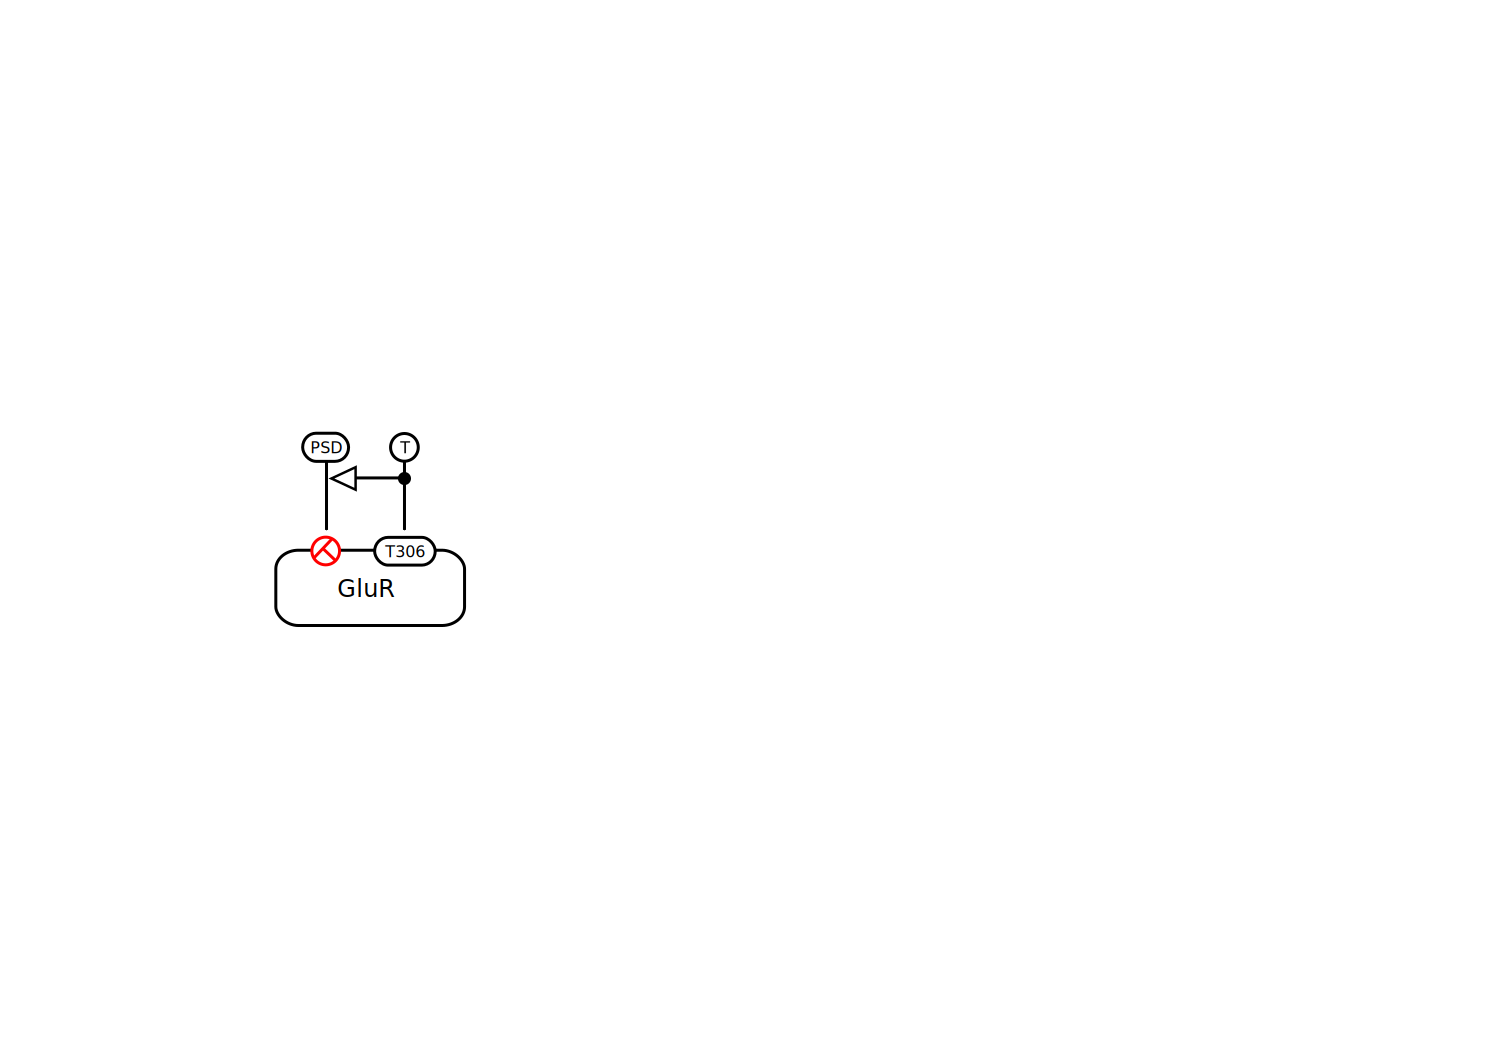
\includegraphics[scale = 0.5]{examples/ex-location-2}
  \caption{Using the \glyph{state variable} \glyph{location} to represent the fact that phosphorylation of glutamate receptors stimulate their incorporation in the post-synaptic density.}
  \label{fig:ex-location}
\end{figure}

%\normalcolor

% The following is for [X]Emacs users.  Please leave in place.
% Local Variables:
% TeX-master: "../sbgn_ER-level1"
% End:



%% $HeadURL: https://sbgn.svn.sourceforge.net/svnroot/sbgn/trunk/documents/specifications/EntityRelationship/Level1/sources/complex-en-eg.tex $

\subsection{Examples of complex ENs}
\label{sec:CplxENs}

In this section, we provide examples of Entity Node representations drawn using the \SBGNERLone glyphs described above.  The first is a representation of the calcium/calmodulin kinase II, with the phosphorylation sites threonine 286 and 306, as well as catalytic and autoinhibitory domains.  This is shown in \fig{example-camkii}.  Note the use of \emph{units of information} and \emph{state variables}.

\begin{figure}[H]
  \centering
  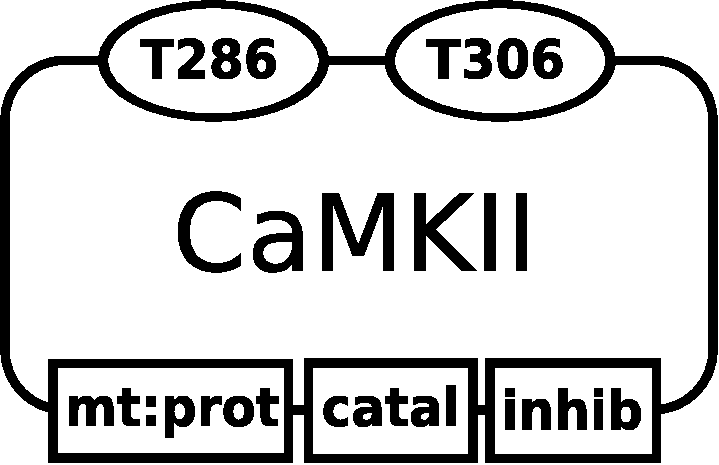
\includegraphics[scale = 0.3]{examples/macromolecule-CaMKII}
  \caption{An example representation of calcium/calmodulin kinase II.}
  \label{fig:example-camkii}
\end{figure}

The next EN example is a representation of the glutamate receptor in with a pore, and with both phosphorylation and glycosylation.  The entity carries two functional domains, the ligand-binding domain and the ion pore.  \fig{example-glur} gives the diagram.

\begin{figure}[H]
  \centering
  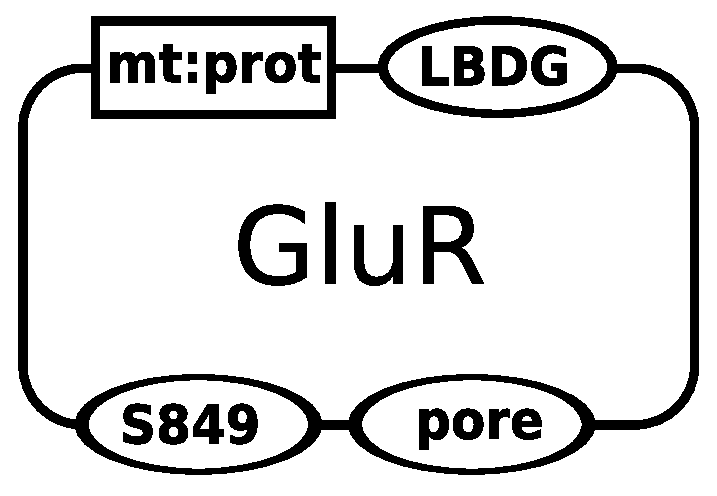
\includegraphics[scale = 0.3]{examples/macromolecule-GluR}
  \caption{An example of a glutamate receptor in the open state.}
  \label{fig:example-glur}
\end{figure}




%%% Local Variables: 
%%% mode: latex
%%% TeX-master: "../sbgn_ER-level1"
%%% End: 

 
%%%%%%%%%%%%%%%%%%%%%%%%%%%%%%%%%%%%%%%%%%%%%%%%%%%%%%%%%%%%%%%%%%%%%%%
%%%%                   Submap
%%%%%%%%%%%%%%%%%%%%%%%%%%%%%%%%%%%%%%%%%%%%%%%%%%%%%%%%%%%%%%%%%%%%%%

\color{red}

A \glyph{submap} is used to encapsulate entities and relationships (including all types of nodes and edges) within one named glyph. The content of the submap can be found for instance on another (web) page in the case of static maps, or can be displayed dynamicaly. Because of the independence of rules, no particular connections are needed between the submap and the containing map.

\begin{figure}[H]
  \centering
  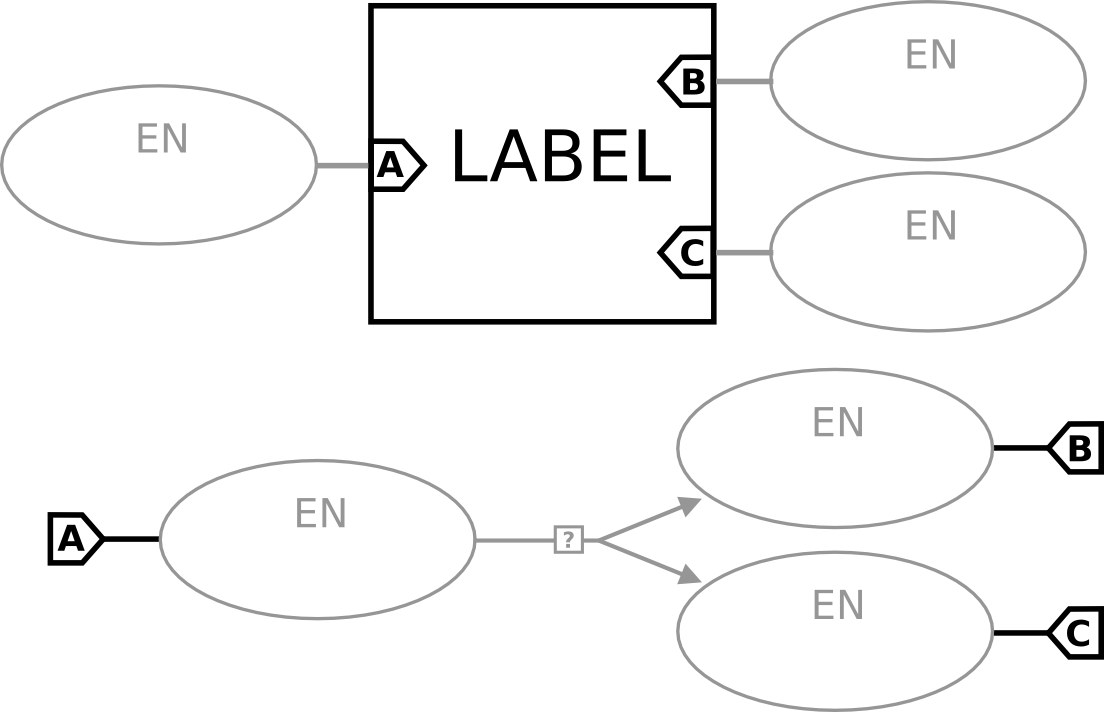
\includegraphics[scale = 0.3]{images/submap}
  \caption{The \ER glyph for \glyph{submap}.}
  \label{fig:submap}
\end{figure}


\normalcolor


%%%%%%%%%%%%%%%%%%%%%%%%%%%%%%%%%%%%%%%%%%%%%%%%%%%%%%%%%%%%%%%%%%%%%%
%%%%%%%%%%%%%%%%%%%%%%%%%%%%%%%%%%%%%%%%%%%%%%%%%%%%%%%%%%%%%%%%%%%%%%
%%%%                   Process nodes
%%%%%%%%%%%%%%%%%%%%%%%%%%%%%%%%%%%%%%%%%%%%%%%%%%%%%%%%%%%%%%%%%%%%%%
%%%%%%%%%%%%%%%%%%%%%%%%%%%%%%%%%%%%%%%%%%%%%%%%%%%%%%%%%%%%%%%%%%%%%%
 
%\section{Process nodes}\label{sec:PNs}

%Process nodes represent processes that transform one or several ENs into one or several different ENs.
 
%% $HeadURL: https://sbgn.svn.sourceforge.net/svnroot/sbgn/trunk/documents/specifications/EntityRelationship/Level1/sources/transition.tex $

%%%%%%%%%%%%%%%%%%%%%%%%%%%%%%%%%%%%%%%%%%%%%%%%%%%%%%%%%%%%%%%%%%%%%%
%%                     Transition
%%%%%%%%%%%%%%%%%%%%%%%%%%%%%%%%%%%%%%%%%%%%%%%%%%%%%%%%%%%%%%%%%%%%%%
\color{red}
\subsection{Glyph: \glyph{Transition}}
\label{sec:transition}

A transition is a process transforming a set of entities (represented by \glyph{ENs} in \SBGNPDLone) into another set entities.

\begin{glyphDescription}

\glyphSboTerm SBO:0000167 ! reaction

\glyphOrigin One or several \glyph{consumption} arcs (\sect{consumption}) or one or several \glyph{production} arcs (\sect{production}).

\glyphTarget One or several \glyph{production} arcs (\sect{production}).

\glyphNode A transition is represented by a square box linked to two connectors, small arcs attached to the centers of opposite sides. The consumption (\sect{consumption}) and production (\sect{production}) arcs are linked to the extremities of those connectors. The modulatory arcs (\sect{arcs}) point to the other two sides of the box. A \glyph{transition} connected to \glyph{production} arcs on opposite sides is a reversible transition. The connectors and the box move as a rigid entity.

\end{glyphDescription}

\begin{figure}[H]
  \centering
  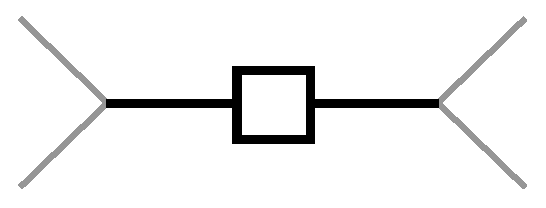
\includegraphics[scale = 0.4]{images/transition}
  \caption{The \ER glyph for \glyph{transition}.}
  \label{fig:transition}
\end{figure}

A transition is the basic process node in SBGN.  It describes a process that transforms a given set of biochemical entities---macromolecules, simple chemicals or unspecified entities---into another set of biochemical entities.  Such a transformation might imply modification of covalent bonds (conversion), modification of the relative position of constituents (conformational transition) or movement from one compartment to another (translocation).

A cardinality label may be associated with \glyph{consumption} (\sect{consumption}) or \glyph{production} (\sect{production}) arcs to indicate the stoichiometry of the process.  This label becomes a requirement when the exact composition of the number of copies of the inputs or outputs to a reaction are ambiguous in the diagram.

The example in \fig{trans-react} illustrates the use of a \glyph{transition} node to represent a reaction between two reactants that generates three products. 

\begin{figure}[H]
  \centering
  \includegraphics[scale = 0.3]{examples/transition-reaction}
  \caption{A reaction that generates three products.}
  \label{fig:trans-react}
\end{figure}
 
% SHOULD BECOME AN ASSIGNMENT
%
% The example in \fig{trans-trans} illustrates the use of a \glyph{transition} node to represent a translocation. The large round-cornered rectangle represents a compartment border (see \sect{compartment}).
% 
% \begin{figure}[H]
%   \centering
%   \includegraphics[scale = 0.3]{examples/transition-translocation}
%   \caption{A translocation.}
%   \label{fig:trans-trans}
% \end{figure}

\normalcolor

% The following is for [X]Emacs users.  Please leave in place.
% Local Variables:
% TeX-master: "../sbgn_ER-level1"
% End:

%\input{sources/omitted.tex}
%\input{sources/uncertain.tex}

% %%%%%%%%%%%%%%%%%%%%%%%%%%%%%%%%%%%%%%%%%%%%%%%%%%%%%%%%%%%%%%%%%%%%%%
% %%%%%%%%%%%%%%%%%%%%%%%%%%%%%%%%%%%%%%%%%%%%%%%%%%%%%%%%%%%%%%%%%%%%%%
% %%%%                  Arcs
% %%%%%%%%%%%%%%%%%%%%%%%%%%%%%%%%%%%%%%%%%%%%%%%%%%%%%%%%%%%%%%%%%%%%%%
% %%%%%%%%%%%%%%%%%%%%%%%%%%%%%%%%%%%%%%%%%%%%%%%%%%%%%%%%%%%%%%%%%%%%%%
 
%\section{Connecting arcs}\label{sec:arcs}

%Connecting arcs are lines that link EPNs and PNs together. The symbols attached to their extremities precise their semantics.
 
% \input{sources/consumption.tex}
% \input{sources/production.tex}
% %\input{sources/truth.tex}
% %%%%%%%%%%%%%%%%%%%%%%%%%%%%%%%%%%%%%%%%%%%%%%%%%%%%%%%%%%%%%%%%%%%%%%
%%                     Modulation
%%%%%%%%%%%%%%%%%%%%%%%%%%%%%%%%%%%%%%%%%%%%%%%%%%%%%%%%%%%%%%%%%%%%%%
\color{blue}
\subsubsection{Glyph: \glyph{Modulation}}\label{sec:modulation}

A modulation affects the strength, or the probability to exist, of the target relationship. Such a modulation can affect the relationship \textbf{positively or negatively}, or even both ways depending on the conditions. A \glyph{modulation} can also be used when one does not know the precise direction of the effect, for instance if there are conflicting evidence.

\begin{glyphDescription}
 \glyphSboTerm SBO:0000168 ! control.
 \glyphOrigin Any \glyph{entity node} (\sect{ENs}).
 \glyphTarget Any \glyph{relationship} (\sect{relationships}).
 \glyphEndPoint The target extremity of a \glyph{modulation} carries an empty diamond.
 \end{glyphDescription}

\begin{figure}[H]
  \centering
  
\includegraphics[scale = 0.5]{images/modulation}
  \caption{The \ER glyph for \glyph{modulation}.}
  \label{fig:modulation}
\end{figure}
 
\begin{figure}[H]
  \centering
  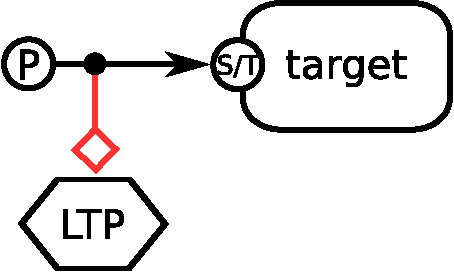
\includegraphics[scale = 0.5]{examples/ex-modulation}
  \caption{Example of a \glyph{modulation} of the \glyph{phenotype} ``Long Term Potentiation (LTP)'' by the phosphorylation of an \glyph{entity} ``target''. For instance the influence could be positive (stimulation, see \sect{stimulation}) or negative (inhibition, see \sect{inhibition}).}
  \label{fig:ex-modulation}
\end{figure}

\normalcolor


% %%%%%%%%%%%%%%%%%%%%%%%%%%%%%%%%%%%%%%%%%%%%%%%%%%%%%%%%%%%%%%%%%%%%%%
%%                     Stimulation
%%%%%%%%%%%%%%%%%%%%%%%%%%%%%%%%%%%%%%%%%%%%%%%%%%%%%%%%%%%%%%%%%%%%%%

\subsubsection{Glyph: \glyph{Stimulation}}\label{sec:stimulation}
\color{blue}

A \glyph{stimulation} affects \textbf{positively} the strength, or the probability, of the target relationship. This stimulation can be for instance a catalysis or a positive allosteric regulation.

\begin{glyphDescription}
 \glyphSboTerm SBO:0000170 ! stimulation.
 \glyphOrigin Any \glyph{entity node} (\sect{ENs}).
 \glyphTarget Any \glyph{relationship} (\sect{relationships}).
 \glyphEndPoint The target extremity of a \glyph{stimulation} carries an empty arrowhead.
 \glyphAux A \glyph{unit of information} carrying the mention \glyph{cis} or \glyph{trans} precises the relationship between the \glyph{entity node} from which the \glyph{stimulation} origins and either:
\begin{itemize}
\item the \glyph{entity node} from which the influence targeted by the \glyph{stimulation} origins
\item all the relevant \glyph{interactors} of the \glyph{interaction} or the \glyph{non-interaction} targeted by the \glyph{stimulation}
\item the \glyph{entity} subjected to the \glyph{assignment} targeted by the \glyph{stimulation}
\end{itemize}
 \end{glyphDescription}

\begin{figure}[H]
  \centering
  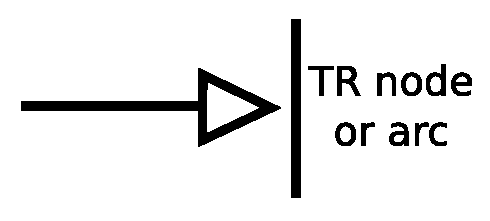
\includegraphics[scale = 0.5]{images/stimulation}
  \caption{The \PD glyph for \glyph{stimulation}.}
  \label{fig:stimulation}
\end{figure}

\begin{figure}[H]
  \centering
  \includegraphics[scale = 0.5]{examples/ex-stimulation}
  \caption{Example of a \glyph{stimulation} a \glyph{phenotype} ``Long Term Potentiation (LTP)'' enhanced when the entity ``GluR'' is present in the post-synaptic density.}
  \label{fig:ex-stimulation}
\end{figure}

\normalcolor




% \input{sources/catalysis.tex}
% %%%%%%%%%%%%%%%%%%%%%%%%%%%%%%%%%%%%%%%%%%%%%%%%%%%%%%%%%%%%%%%%%%%%%%
%%                     Inhibition
%%%%%%%%%%%%%%%%%%%%%%%%%%%%%%%%%%%%%%%%%%%%%%%%%%%%%%%%%%%%%%%%%%%%%%

\subsubsection{Glyph: \glyph{Inhibition}}\label{sec:inhibition}
\color{blue}

An inhibition \textbf{negatively}  the strength, or the probability, of the target relationship. This inhibition can be for instance a steric hindrance or a negative allosteric regulation.

\begin{glyphDescription}
 \glyphSboTerm SBO:0000170 ! inhibition.
 \glyphOrigin Any \glyph{entity node} (\sect{ENs}).
 \glyphTarget Any \glyph{relationship} (\sect{relationships}).
 \glyphEndPoint The target extremity of a \glyph{inhibition} carries a bar perpendicular to the arc.
 \end{glyphDescription}

\begin{figure}[H]
  \centering
  \includegraphics[scale = 0.3]{images/inhibition}
  \caption{The \PD glyph for \glyph{inhibition}.}
  \label{fig:inhibition}
\end{figure}

\begin{figure}[H]
  \centering
  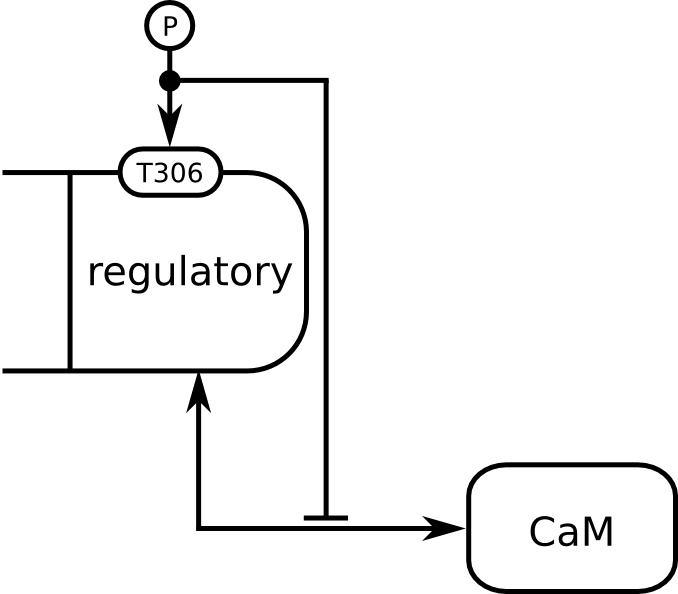
\includegraphics[scale = 0.5]{examples/ex-inhibition}
  \caption{In this example, the phosphorylation of the threonine 306 of the regulatory domain of CaMKII inhibits the interaction between Calmodulin and the kinase.}
  \label{fig:ex-inhibition}
\end{figure}

\normalcolor


% \input{sources/trigger.tex}
% %%%%%%%%%%%%%%%%%%%%%%%%%%%%%%%%%%%%%%%%%%%%%%%%%%%%%%%%%%%%%%%%%%%%%%
%%                     Logic arc
%%%%%%%%%%%%%%%%%%%%%%%%%%%%%%%%%%%%%%%%%%%%%%%%%%%%%%%%%%%%%%%%%%%%%%
%\color{blue}
\subsubsection{Glyph: \glyph{Logic arc} }\label{sec:logicArc}

\glyph{Logic arc} is used to represent the fact that an interactor influences
the outcome of a logic operator. 

\begin{glyphDescription}
 \glyphSboTerm SBO:0000398 - logical relationship.
 \glyphOrigin Any \glyph{interactor} (\sect{interactors}) or \glyph{logical operator} (\sect{logic}).
 \glyphTarget Any \glyph{logical operator} (\sect{logic}).
 \glyphEndPoint No particular symbol is used to represent a logic arc.
 \end{glyphDescription}

\begin{figure}[H]
  \centering
  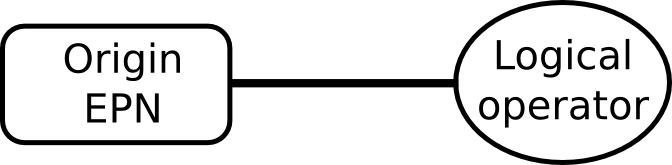
\includegraphics[scale = 0.4]{images/logicArc}
  \caption{The \ER glyph for \glyph{logic arc}.}
  \label{fig:logicArc}
\end{figure}

\begin{figure}[H]
  \centering
  \includegraphics[scale = 0.5]{examples/ex-logicArc}
  \caption{In this example, two logic arcs reflect the fact that the phosphorylation of threonine 306 on CaMKII is precluded either by a dimerisation or the binding of calmodulin.}
  \label{fig:ex-logicArc}
\end{figure}

%\normalcolor
% \input{sources/equivalenceArc.tex}

% %%%%%%%%%%%%%%%%%%%%%%%%%%%%%%%%%%%%%%%%%%%%%%%%%%%%%%%%%%%%%%%%%%%%%%
% %%%%%%%%%%%%%%%%%%%%%%%%%%%%%%%%%%%%%%%%%%%%%%%%%%%%%%%%%%%%%%%%%%%%%%
% %%%%                  Relashionships
% %%%%%%%%%%%%%%%%%%%%%%%%%%%%%%%%%%%%%%%%%%%%%%%%%%%%%%%%%%%%%%%%%%%%%%
% %%%%%%%%%%%%%%%%%%%%%%%%%%%%%%%%%%%%%%%%%%%%%%%%%%%%%%%%%%%%%%%%%%%%%%

% \section{Relationships}\label{sec:relationships}

% Assignment
% Interaction
% Self
% 
% %%%%%%%%%%%%%%%%%%%%%%%%%%%%%%%%%%%%%%%%%%%%%%%%%%%%%%%%%%%%%%%%%%%%%%
% %%%%%%%%%%%%%%%%%%%%%%%%%%%%%%%%%%%%%%%%%%%%%%%%%%%%%%%%%%%%%%%%%%%%%%
% %%%%                   Logical operators
% %%%%%%%%%%%%%%%%%%%%%%%%%%%%%%%%%%%%%%%%%%%%%%%%%%%%%%%%%%%%%%%%%%%%%%
% %%%%%%%%%%%%%%%%%%%%%%%%%%%%%%%%%%%%%%%%%%%%%%%%%%%%%%%%%%%%%%%%%%%%%%
% 
% \section{Logical operators}\label{sec:logic}
% 
% %%%%%%%%%%%%%%%%%%%%%%%%%%%%%%%%%%%%%%%%%%%%%%%%%%%%%%%%%%%%%%%%%%%%%%
%%                     And
%%%%%%%%%%%%%%%%%%%%%%%%%%%%%%%%%%%%%%%%%%%%%%%%%%%%%%%%%%%%%%%%%%%%%%
\color{blue}
\subsubsection{Glyph: \glyph{And}}\label{sec:and}

The glyph \glyph{and} is used to denote that all the \glyph{entity nodes} linked as input are necessary to produce the output influence.

\begin{glyphDescription}

 \glyphSboTerm SBO:0000173 ! and.

 \glyphContainer \glyph{And} is represented by a circle, with two connectors located at the opposite side for inputs and output.

  \glyphLabel \glyph{And} is identified by the label ``AND'' placed in an unbordered box attached to the center of the container. 

  \glyphAux \glyph{And} does not carry any auxiliary items.

\end{glyphDescription}


\begin{figure}[H]
  \centering
  \includegraphics[scale = 0.5]{images/and}
  \caption{The \ER glyph for \glyph{and}. Three inputs are represented, but two or more than three would be allowed.}
  \label{fig:and}
\end{figure}


% The following diagrams illustrate the dephosphorylation of the MAP inase ERK by the protein phosphatase 2A and the STriatal Enriched Phosphatase, in ST (left) and ER (right).
%
% \begin{center}
% \scalebox{0.5}{\includegraphics{images/stimulation-example1}}
% \end{center}
\normalcolor

% %%%%%%%%%%%%%%%%%%%%%%%%%%%%%%%%%%%%%%%%%%%%%%%%%%%%%%%%%%%%%%%%%%%%%%
%%                     Or
%%%%%%%%%%%%%%%%%%%%%%%%%%%%%%%%%%%%%%%%%%%%%%%%%%%%%%%%%%%%%%%%%%%%%%
\color{blue}
\subsection{Glyph: \glyph{Or}}\label{sec:or}

The glyph \glyph{or} is used to denote that any of the \glyph{interactor nodes} linked as input is sufficient to produce the output influence.

\begin{glyphDescription}
 \glyphSboTerm SBO:0000174 ! or.
 \glyphOrigin One interactor (section~\ref{sec:interactors}) or logical operator (section~\ref{sec:logic}).
 \glyphTarget  One modulation (section~\ref{sec:modulation}), stimulation (section~\ref{sec:stimulation}), inhibition (section~\ref{sec:inhibition}), necessary  stimulation (section~\ref{sec:necessaryStimulation}), or absolute inhibition (section~\ref{sec:absoluteInhibition}) arc.
 \glyphNode \glyph{Or} is represented by a circle carrying the word ``OR''.
 \end{glyphDescription}

\begin{figure}[H]
  \centering
  \includegraphics[scale = 0.5]{images/or}
  \caption{The \ER glyph for \glyph{or}. Only two inputs are represented, but more would be allowed.}
  \label{fig:or}
\end{figure}



% %%%%%%%%%%%%%%%%%%%%%%%%%%%%%%%%%%%%%%%%%%%%%%%%%%%%%%%%%%%%%%%%%%%%%%
%%                     Not
%%%%%%%%%%%%%%%%%%%%%%%%%%%%%%%%%%%%%%%%%%%%%%%%%%%%%%%%%%%%%%%%%%%%%%
\color{blue}
\subsubsection{Glyph: \glyph{Not}}\label{sec:not}

The glyph \glyph{not} is used to denote that the output influence only happen in the absence of the input \glyph{interactor}.

\begin{glyphDescription}

 \glyphSboTerm SBO:0000238 ! not.

 \glyphContainer \glyph{Not} is represented by a circle, with two connectors located at the opposite side for input and output.

  \glyphLabel \glyph{Not} is identified by the label ``NOT'' placed in an unbordered box attached to the center of the container. 

  \glyphAux \glyph{Not} does not carry any auxiliary items.

\end{glyphDescription}

\begin{figure}[H]
  \centering
  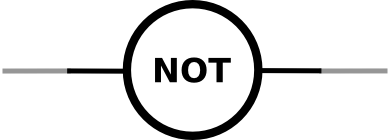
\includegraphics[scale = 0.5]{images/not}
  \caption{The \ER glyph for \glyph{not}.}
  \label{fig:not}
\end{figure}






% The following is for [X]Emacs users.  Please leave in place.
% Local Variables:
% TeX-master: "../sbgn_ER-level1"
% End:
